% Search for all the places that say "PUT SOMETHING HERE".

\documentclass[11pt]{article}
\usepackage{amsmath,textcomp,amssymb,geometry,graphicx,enumerate}

\def\Name{Ran Liao}  % Your name
\def\SID{3034504227}  % Your student ID number
\def\Homework{3} % Number of Homework
\def\Session{Spring 2019}


\title{CS170--Spring 2019 --- Homework \Homework\ Solutions}
\author{\Name, SID \SID}
\markboth{CS170--\Session\  Homework \Homework\ \Name}{CS170--\Session\ Homework \Homework\ \Name}
\pagestyle{myheadings}
\date{\today}

\newenvironment{qparts}{\begin{enumerate}[{(}a{)}]}{\end{enumerate}}
\def\endproofmark{$\Box$}
\newenvironment{proof}{\par{\bf Proof}:}{\endproofmark\smallskip}

\textheight=9in
\textwidth=6.5in
\topmargin=-.75in
\oddsidemargin=0.25in
\evensidemargin=0.25in


\begin{document}
\maketitle
Collaborators: Yilin Wu, Jingyi Xu, Renee Pu

\section{Study Group}
	\begin{tabular}{ll}
		Name		&   SID         		\\\hline
		Ran Liao		&   3034504227  	\\  
		Yilin Wu		&   3034503863  	\\
		Jingyi Xu		&   3032003885  	\\
		Renee Pu		&   3032083302  	\\
	\end{tabular}



\newpage
\section{Maximum Subarray Sum}

\begin{qparts}
	\item \textbf{Description}

	This algorithm will scan the array twice to find the answer.
		
	Assume index starts with 0. Let $A[i]$ be the $i$th element in input array, and $d[i]$ be the maximum sum of subarrays that ends with index $i$. This array will be calculated during the first scan. First, let $d[0]$ equals to $A[0]$. Then, iterate variable $i$ from 1 to $n-1$. If the sum of $d[i-1]$ and $A[i]$ is larger than $A[i]$, assign $d[i]$ with $d[i-1] + A[i]$. Otherwise, assign it with $A[i]$. In the second scan, we can retrieve the maximum value in $d$ array, and that is the answer.
	
	\item \textbf{Proof of Correctness}
	
	Before iteration, $d[0]$ equals to$A[0]$. This is indeed the maximum sum of subarray that ends with index 0, which contains only the first element. During iteration, there're only two possible situations. Either (1) append $A[i]$ to the maximum subarray that ends with $A[i-1]$ will result a larger sum, or (2) a subarray that contains only $A[i]$ itself will result to a better solution. Therefore, by taking the maximum value between $d[i-1] + A[i]$ and $A[i]$, we will guarantee the correctness of $d[i]$. Therefore, we can guarantee the correctness of first scan. And in the second scan, the largest value in array $d$ will be considered as the final answer. This value must be correct because it is the maximum possible sum of subarrays no matter where it ends.
	
	\item \textbf{Runtime Analysis}
	
	This algorithm takes only 2 scan, each of them will cost $O(n)$ time. So the total runtime is $O(n)$.

\end{qparts}

\newpage
\section{Modular Fourier Transform}

\begin{qparts}
	\item 
	\[
		1 * 1 * 1 * 1 = 1 \equiv 1 (\operatorname{mod}) 5
	\]
	\[
		2 * 2 * 2 * 2 = 16 \equiv 1 (\operatorname{mod}) 5
	\]
	\[
		3 * 3 * 3 * 3 = 81 \equiv 1 (\operatorname{mod}) 5
	\]
	\[
		4 * 4 * 4 * 4 = 256 \equiv 1 (\operatorname{mod}) 5
	\]
	\[
		1 + \omega +  \omega^2 + \omega^3 = 1 + 2 + 4 + 8 = 15 \equiv 0 (\operatorname{mod})5
	\]

	\item
	\[
		\vec u = M_4(\omega)\vec v
		= 
		\begin{bmatrix} 
			1 & 1 & 1 & 1 \\ 
			1 & \omega^1 & \omega^2 & \omega^3 \\ 
			1 & \omega^2 & \omega^4 & \omega^6 \\ 
			1 & \omega^3 & \omega^6 & \omega^9 \\ 
		\end{bmatrix}
		\begin{bmatrix} 
			0 \\ 
			1 \\ 
			0 \\ 
			2 \\ 
		\end{bmatrix} 
		=
		\begin{bmatrix} 
			1 & 1 & 1 & 1 \\ 
			1 & 2 & 4 & 3 \\ 
			1 & 4 & 1 & 4 \\ 
			1 & 3 & 4 & 2 \\ 
		\end{bmatrix}		
		\begin{bmatrix} 
			0 \\ 
			1 \\ 
			0 \\ 
			2 \\ 
		\end{bmatrix} 
		=
		\begin{bmatrix} 
			3 \\ 
			3 \\ 
			2 \\ 
			2 \\ 
		\end{bmatrix}
	\]

	\item
	\[
		\vec v = \frac{1}{4}M_4(\omega^{-1})\vec u
		= 
		\frac{1}{4}
		\begin{bmatrix} 
			1 & 1 & 1 & 1 \\ 
			1 & \omega^{-1} & \omega^{-2} & \omega^{-3} \\ 
			1 & \omega^{-2} & \omega^{-4} & \omega^{-6} \\ 
			1 & \omega^{-3} & \omega^{-6} & \omega^{-9} \\ 
		\end{bmatrix}
		\begin{bmatrix} 
			3 \\ 
			3 \\ 
			2 \\ 
			2 \\ 
		\end{bmatrix}
		=
		\frac{1}{4}
		\begin{bmatrix} 
			1 & 1 & 1 & 1 \\ 
			1 & 3 & 4 & 2 \\ 
			1 & 4 & 1 & 4 \\ 
			1 & 2 & 4 & 3 \\ 
		\end{bmatrix}		
		\begin{bmatrix} 
			3 \\ 
			3 \\ 
			2 \\ 
			2 \\ 
		\end{bmatrix}
		=
		\frac{1}{4}
		\begin{bmatrix} 
			0 \\ 
			4 \\ 
			0 \\ 
			3 \\ 
		\end{bmatrix}
		=
		\begin{bmatrix} 
			0 \\ 
			1 \\ 
			0 \\ 
			2 \\ 
		\end{bmatrix} 
	\]
	
	\item
	The given two polynomials can be written into the following form.
	\[
		2x^2 + 3 \equiv (3 + 0x + 2x^2 + 0x^3)(\operatorname{mod})5
	\]
	\[
		-x + 3 \equiv (3 + 4x + 0x^2 + 0x^3)(\operatorname{mod})5
	\]
	Let $\vec a$ be $[3, 0, 2, 0]^T$,  and $\vec b$ be $[3, 4, 0, 0]^T$. 
	
	First, perform FT with $\vec a$ and $\vec b$.
	\[
		\vec a^\prime = M_4(\omega)\vec a
		= 
		\begin{bmatrix} 
			1 & 1 & 1 & 1 \\ 
			1 & \omega^1 & \omega^2 & \omega^3 \\ 
			1 & \omega^2 & \omega^4 & \omega^6 \\ 
			1 & \omega^3 & \omega^6 & \omega^9 \\ 
		\end{bmatrix}
		\begin{bmatrix} 
			3 \\ 
			0 \\ 
			2 \\ 
			0 \\ 
		\end{bmatrix}
		=
		\begin{bmatrix} 
			1 & 1 & 1 & 1 \\ 
			1 & 2 & 4 & 3 \\ 
			1 & 4 & 1 & 4 \\ 
			1 & 3 & 4 & 2 \\ 
		\end{bmatrix}		
		\begin{bmatrix} 
			3 \\ 
			0 \\ 
			2 \\ 
			0 \\ 
		\end{bmatrix}
		=
		\begin{bmatrix} 
			0 \\ 
			1 \\ 
			0 \\ 
			1 \\ 
		\end{bmatrix}
	\]
	\[
		\vec b^\prime = M_4(\omega)\vec b
		= 
		\begin{bmatrix} 
			1 & 1 & 1 & 1 \\ 
			1 & \omega^1 & \omega^2 & \omega^3 \\ 
			1 & \omega^2 & \omega^4 & \omega^6 \\ 
			1 & \omega^3 & \omega^6 & \omega^9 \\ 
		\end{bmatrix}
		\begin{bmatrix} 
			3 \\ 
			4 \\ 
			0 \\ 
			0 \\ 
		\end{bmatrix}
		=
		\begin{bmatrix} 
			1 & 1 & 1 & 1 \\ 
			1 & 2 & 4 & 3 \\ 
			1 & 4 & 1 & 4 \\ 
			1 & 3 & 4 & 2 \\ 
		\end{bmatrix}		
		\begin{bmatrix} 
			3 \\ 
			4 \\ 
			0 \\ 
			0 \\ 
		\end{bmatrix}
		=
		\begin{bmatrix} 
			2 \\ 
			1 \\ 
			4 \\ 
			0 \\ 
		\end{bmatrix}
	\]
	Second, multiply $\vec a^\prime$ and $\vec b^\prime$ elementwise.
	\[
		\vec c^\prime = \vec a^\prime * \vec b^\prime = 
		\begin{bmatrix} 
			0 \\ 
			1 \\ 
			0 \\ 
			1 \\ 
		\end{bmatrix}
		*
		\begin{bmatrix} 
			2 \\ 
			1 \\ 
			4 \\ 
			0 \\ 
		\end{bmatrix}
		=
		\begin{bmatrix} 
			0 \\ 
			1 \\ 
			0 \\ 
			0 \\ 
		\end{bmatrix}
	\]
	Then, perform inverse FT with $\vec c^\prime$.
	\[
		\vec c = \frac{1}{4}M_4(\omega^{-1})\vec c^\prime
		= 
		\frac{1}{4}
		\begin{bmatrix} 
			1 & 1 & 1 & 1 \\ 
			1 & \omega^{-1} & \omega^{-2} & \omega^{-3} \\ 
			1 & \omega^{-2} & \omega^{-4} & \omega^{-6} \\ 
			1 & \omega^{-3} & \omega^{-6} & \omega^{-9} \\ 
		\end{bmatrix}
		\begin{bmatrix} 
			0 \\ 
			1 \\ 
			0 \\ 
			0 \\ 
		\end{bmatrix}
		=
		\frac{1}{4}
		\begin{bmatrix} 
			1 & 1 & 1 & 1 \\ 
			1 & 3 & 4 & 2 \\ 
			1 & 4 & 1 & 4 \\ 
			1 & 2 & 4 & 3 \\ 
		\end{bmatrix}		
		\begin{bmatrix} 
			0 \\ 
			1 \\ 
			0 \\ 
			0 \\ 
		\end{bmatrix}
		=
		\frac{1}{4}
		\begin{bmatrix} 
			1 \\ 
			3 \\ 
			4 \\ 
			2 \\ 
		\end{bmatrix}
		=
		\begin{bmatrix} 
			4 \\ 
			2 \\ 
			1 \\ 
			3 \\ 
		\end{bmatrix} 
	\]
	Therefore, we get the answer $4 + 2x + x^2 + 3x^3$, which of course is with respective to module 5.
\end{qparts}

\newpage
\section{Polynomial from roots}

\begin{qparts}
	\item \textbf{Main Idea}
	
	This problem is equivalent to compute coefficients of expression $\prod_{i=1}^{n}(x - r_i)$, which is actually the product of $n$ polynomials. The idea is split this expression into 2 components with equal length recursively, solve these 2 subexpressions and multiply them together to get the final answer. 
	
	\item \textbf{Runtime Analysis}
	
	The algorithm will use divide and conquer strategy. Specifically, it will split the original expression into 2 equal length subexpressions.  And it will use FFT to multiply 2 sub-expression together, which will cost $O( \frac{n}{2}\log \frac{n}{2})$ time. Therefore, we have the following recursive formula:
	\begin{align*}
		T(n) &= 2T(\frac{n}{2}) + \frac{n}{2}\log \frac{n}{2} \\
		&= 2^2T(\frac{n}{2^2}) + \frac{n}{2}\log \frac{n}{2} + \frac{n}{2}\log \frac{n}{2^2} \\
		&= 2^kT(\frac{n}{2^k}) + \frac{n}{2}\log \frac{n}{2} + \frac{n}{2}\log \frac{n}{2^2} + \ldots + \frac{n}{2}\log \frac{n}{2^k} \\
		&= 2^{\log n}T(\frac{n}{2^{\log n}}) + \frac{n}{2}\log \frac{n}{2} + \frac{n}{2}\log \frac{n}{2^2} + \ldots + \frac{n}{2}\log \frac{n}{2^{\log n}} \\
		&= n + \frac{n}{2}(\log \frac{n}{2} + \log \frac{n}{2^2} + \ldots + \log \frac{n}{2^{\log n}}) \\
		&= n + \frac{n}{2} \log ({\frac{n^{\log n}}{2^{\frac{(1 + \log n)\log n}{2}}}}) \\
		&= n + \frac{n\log n}{2} \log ({\frac{n}{2^{\frac{(1 + \log n)}{2}}}}) \\
		&= n + \frac{n\log n}{2} (\log n - \frac{(1 + \log n)}{2} \log 2) \\
		&= n + \frac{n\log^2 n}{2} - \frac{ n\log n (1 + \log n)}{4}  \\
		&= n + \frac{n\log^2 n}{4} - \frac{ n\log n }{4}  \\
		&= O(n \log^2 n)
	\end{align*}
\end{qparts}
	
\newpage
\section{Triple sum}

\begin{qparts}
	\item \textbf{Main Idea}
	
	We can construct the following polynomial $P$ base on elements in array $A$.
	
	\[
		P = \sum_{i=0}^{n-1} x^{A[i]}
	\]
	
	Then we compute $P^3$ using FFT. Index $i, j, k$ exists if and only if the coefficient of $x^n$ in $P^3$ is not 0.
	
	\item \textbf{Pseudocode}
	
	IF-INDEX-EXIST($A$)\{
	
		\qquad $n \leftarrow \operatorname{LEN}(A)$
		
		\qquad $P \leftarrow$ empty array with length $n$, and initialize them with 0
		
		\qquad  for ($i=0;i<n;i++$)\{
					
		\qquad\qquad $P[A[i]]++$
				
		\qquad \}
		
		\qquad $P^2 \leftarrow$ FFT($P$, $P$)
		
		\qquad $P^3 \leftarrow$ FFT($P^2$, $P$)
		
		\qquad if ( $P_3[n] \neq 0$ ) \{
		
		\qquad\qquad RETURN $True$
		
		\qquad\} else \{
		
		\qquad\qquad RETURN $False$
		
		\qquad\}
		
	\}
	
	\item \textbf{Runtime Analysis}
	
	Construct polynomial $P$ will cost $O(n)$ time, and compute $P^3$ by perform FFT twice will cost $O(n\log n)$ time. Therefore, the total runtime is $O(n\log n)$.
	
	\item \textbf{Proof of Correctness}
	
	\[
		P^3 = \sum_{a=0}^{n-1} \sum_{b=0}^{n-1} \sum_{c=0}^{n-1} P[a] \cdot P[b] \cdot P[c] \cdot x^{a+b+c}
	\]
	
	All coefficients in $P$ is larger than or equal to 0. Therefore, if the coefficient of $x^n$ in $P^3$ is not 0, there exists $a, b, c$ such that $a + b + c = n$ and both $P[a]$, $P[b]$, $P[c]$ are not 0. Notice that if $P[x]$ is not 0, original array $A$ must contain a value that equals to $x$. Hence, the original array must contain value that equals to $a, b, c$ respectively, and these three values have sum equals to $n$.
	
\end{qparts}

\newpage
\section{Searching for Viruses}

\begin{qparts}

	\item 
	\renewcommand{\theenumii}{\roman{enumii}}
	\begin{enumerate}
		\item \textbf{Main Idea}
		
		This is a brute force algorithm. Possible match of $s_1$ in $s_2$ can start with every position from $0$ to $m-n$. Therefore, I can just iterate through all of it, and check whether the next $n$ characters differ in at most $k$ locations.
		
		\item \textbf{Runtime Analysis}
		
		There're at most $m$ possible starting locations, and checking each of them will cost $O(n)$ time. Therefore, the runtime is $O(nm)$.
		
		\item \textbf{Proof of Correctness}
		
		The correctness of a brute force algorithm is obvious and trivial.
	\end{enumerate}
	
	\item 
	\renewcommand{\theenumii}{\roman{enumii}}
	\begin{enumerate}
		\item \textbf{Description}
		
		I will assume string $s_1$ and $s_2$ are binary string that contain only 0 and 1.  This will not affect the correctness of this algorithm, since all real word characters can be interpreted as a 8-bits binary sequence.
		
		First, I'd like to define this problem more formally.  Denote $P(x)$ as a function that receive an integer index $x$ and give us another integer. The following is the formal expression of $P(x)$.
		\[
			P(x) = \sum_{i=0}^{n-1} (s_1[i] - s_2[x-n+1+i])^2 
		\]		
		Therefore, we have the following deduction:
		\begin{equation}
			\label{eq:proposition}
			P(x) \leq k \iff s_2 \text{ matches } s_1 \text{ from index } x-n+1 \text{ to } x
		\end{equation}
		This is true because I assume all characters are either 0 or 1. Therefore, each time $s_2$ differs from $s_1$ will increase the value of corresponding $P(x)$ by 1.
	
		The whole problem is hence equivalent to \textbf{find all possible $x$ that make $P(x) \leq k$}.
		
		To simplified $P(x)$, denote $s_m$ as the string that is mirror with $s_1$. This property can be expressed like this:
		\[
			s_m[i] = s_1[n-1-i] \quad \forall \ 0 \leq i \leq n-1 
		\]
		Therefore $P(x)$ can be expressed like this:
		\begin{align*}
			P(x) &= \sum_{i=0}^{n-1} \bigg [ s_m[n-1-i] - s_2[x-n+1+i]\bigg ]^2 \\
			&= \sum_{i=0}^{n-1} \bigg [ (s_m[n-1-i])^2 - 2s_m[n-1-i]s_2[x-n+1+i] + (s_2[x-n+1+i])^2 \bigg ] \\
			&=  \sum_{i=0}^{n-1}(s_m[n-1-i])^2 - 2\sum_{i=0}^{n-1}\bigg [s_m[n-1-i]s_2[x-n+1+i]\bigg] + \sum_{i=0}^{n-1}(s_2[x-n+1+i])^2  \\
			&=  \sum_{i=0}^{n-1}(s_m[n-1-i]) - 2\sum_{i=0}^{n-1}\bigg [s_m[n-1-i]s_2[x-n+1+i]\bigg] + \sum_{i=0}^{n-1}(s_2[x-n+1+i])  \\
		\end{align*}
		The last step is correct because I assume $s_1$ and $s_2$ are binary string, so their squares are equals to themself. 
		
		In this long expression, $\sum_{i=0}^{n-1}(s_m[n-1-i])$ is irrelevant to $x$ and can be computed within $O(n)$ time.
		
		Denote $s_{ps}$ to be an array that $s_{ps}[i]$ is $\sum_{j=0}^{i}s_2[j]$($ps$ stands for prefix sum). $s_{ps}$ can be computed with the following formula:
		\[
			s_{ps}[i] = s_{ps}[i-1] + s_2[i]
		\]
		This can be done by scanning $s_2$ once. Therefore, it will cost $O(m)$ time. And $\sum_{i=0}^{n-1}(s_2[x-n+1+i])$  will be equal to $s_{ps}[x] - s_{ps}[x-n]$
		
		$\sum_{i=0}^{n-1}\bigg [s_m[n-1-i]s_2[x-n+1+i]\bigg]$ is hard to compute and needs true inspiration. Notice that the sum of the index of $s_m$ and $s_2$ is $x$. This is the property I will use later.
		
		Suppose $A$ and $B$ are the following polynomials. Let $C$ be the product of them.
		\[
			A = a_0 + a_1x + a_2x^2 + \ldots + a_{m-1}x^{m-1}
		\]
		\[
			B = b_0 + b_1x + b_2x^2 + \ldots + b_{m-1}x^{m-1}
		\]
		The coefficient of $C$ can be expressed like this:
		\[
			c_x = \sum_{i=0}^{x}(a_i \cdot b_{x-i})
		\]
		Notice that the sum of subscripts of $a$ and $b$ is $x$, which is exactly identical with the property I mentioned early except that $A$ and $B$ have equal length. Therefore, I define the  string $s\prime_m$ as follows.
		\[
			s\prime_m[i]=
			\begin{cases}
				s_m[i]	& i < n \\
				0		& n \leq i < m \\
			\end{cases}
		\]
		
		Hence, we can consider $s\prime_m$ and $s_2$ to be the coefficients of two polynomial respectively. Then use FFT  and IFFT to compute the coefficient of their product. $c_x$ is the value of $\sum_{i=0}^{n-1}\bigg [s_m[n-1-i]s_2[x-n+1+i]\bigg]$. This will cost $O(m\log m)$ time.
		
		By now $P(x)$ is fully calculable. Then, deduction \eqref{eq:proposition} will give the final answer.
		

		\item \textbf{Runtime Analysis}
		
		Compute the first part of $P(x)$ will cost $O(n)$ time, and compute the third part will cost $O(m)$ time. Perform FFT and IFFT with problem size $m$ will cost $O(m\log m)$ time. In conclusion, the total runtime is $O(m\log m)$
		
		
		
	\end{enumerate}
\end{qparts}

\newpage
\section{Breadth-First Search}

	\begin{center}
	\begin{tabular}{c | c | c}
	\hline
	Step	& Node Processed        &   Queue         \\\hline
	1	&	&   A		\\\hline
	2	&A	&   B-D	\\\hline
	3	&B	&   D-C-E	\\\hline
	4	&D	&   C-E	\\\hline
	5	&C	&   E-F	\\\hline
	6	&E	&   F		\\\hline
	7	&F	&     		\\\hline
	\end{tabular}
	\end{center}


\begin{figure}[h]
\centering
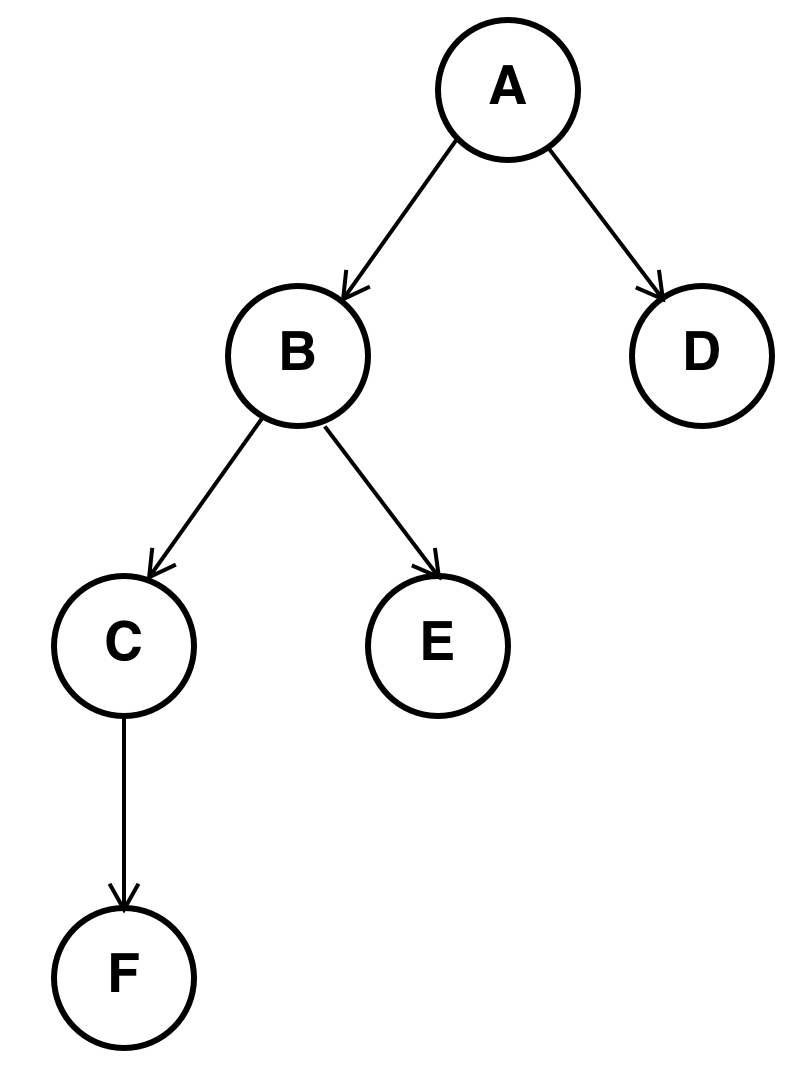
\includegraphics[width=0.5\textwidth]{hw3_bfs.png}
\caption{\label{fig:bfs}BFS Tree}
\end{figure}

\newpage
\section{Breadth-First Search}

\begin{qparts}

	\item \textbf{Main Idea}
	
	First compute the meta-graph $G^M$ of the original graph $G$. Then construct the reverse graph of $G^M$ and denote it as $G^{MR}$. Run DFS algorithm on $G^{MR}$ and record the vertex that has \textbf{largest} \textit{post} number. Denote such vertex as $v_s$. Run \textbf{single} \textit{explore()} function on $v_s$ in graph $G^M$. Vertex $v$ exists if and only if $v_s$ can reach all vertices in $G^{M}$ within this explore.
	
	\item \textbf{Proof of Correctness}
	
	Every pair of vertices can reach each other if they're in the same strong connected component. Therefore, the original proposition is equivalent to check whether a vertex in $G^M$ exists that can reach all other vertices within $G^M$. The vertex with largest \textit{post} number in $G^{MR}$ is a \textit{sink} and hence is a \textit{source} in graph $G^M$. Obviously, this \textit{source} vertex is the only vertex that be possible to reach all other vertices. So just run another \textit{explore()} to check whether it can.
			
	\item \textbf{Runtime Analysis}
	
	Compute the meta-graph $G^M$ will cost $O(|V| + |E|)$ time. Construct the reverse graph $G^{MR}$ also will cost $O(|V| + |E|)$ time. Run DFS search on graph $G^M$ and $G^{MR}$ will still cost $O(|V| + |E|)$ time. Therefore the total runtime is $O(|V|+|E|)$

\end{qparts}


\end{document}